\section{Boundary conditions for fourth-order accuracy}
  

  In this section we discuss some of the issues that arise when solving fourth-order accurate
problems.

Line smoothers require the solution of penta-diagonal systems. We use the {\bf TridiagonalSystem} class
which can solve penta-diagonal systems in addition to tri-diagonal systems.

We use the same restriction and prologonation operators as in the second-order case.

% \subsection{Boundary conditions}

  The multigrid convergence results can be sensitive to the boundary conditions.

For fourth-order accurate discretizations with dirichlet boundary conditions we require
a numerical boundary condition to determine the solution at the first ghost line.

Two possible numerical boundary conditions are
\begin{enumerate}
   \item Extrapolate the ghost line
   \item use the equation on the boundary to second-order
\end{enumerate}
We will consider both these boundary conditions. 
  


\subsection{Neumann and extrapolation boundary conditions}

The most straight forward way to discretize the equations at a boundary with a 
Neumann (or mixed) boundary condition 
\[
   a_1 \partial_n u + a_0 u = g
\]
is to apply the equation and the
Neumann BC to fourth-order on the boundary and to extrapolate the second ghost line.

On a rectangular grid with boundary at $i_1=0$ this would lead to the following two equations
for the 2 ghost point values, $u_{-1}$ and $u_{-2}$,
\begin{align*}
   a_1\Big[ {-u_{-2} + 8 u_{-1} - 8 u_{1} + u_2 \over 12 h } \Big] + a_0 u_0 &= g  \\
   D_+^p u_{-2} &= 0
\end{align*}
Here $p$ is the order of the extrapolation.
For $p=4$ this would give
\begin{align*}
u_{-1} &= \Big( -{3\over 2} - {3 h a_0 \over a_1 } \Big) u_0 + 3 u_1 -{1\over2} u_2 + {3 h \over a_1 } g\\
u_{-2} &= 4 u_{-1} - 6 u_0 + 4 u_1 - u_2
\end{align*}
while for $p=5$,
\begin{align*}
u_{-1} &= \Big( -{10\over 3} - {4 h a_0 \over a_1 } \Big) u_0 + 6 u_1 - 2 u_2 + {1\over 3} u_3 + {4 h \over a_1 } g\\
u_{-2} &= 5 u_{-1} - 10 u_0 + 10 u_1 -5 u_2 + u_3
\end{align*}


On a curvilinear grid the mixed boundary condition would be 
\begin{align*}
    a_1 u_n + a_0 u & = g \\
    a_1 (\nv\cdot\grad_\xv r ) u_r + (\nv\cdot\grad_\xv s ) u_s + (\nv\cdot\grad_\xv t ) u_t & = g
\end{align*}
which is approximated to fourth order using $u_r \approx D_{0r}(1-{h^2\over6} D_{+r}D_{-r}) u$ etc.
The resulting difference approximation can be written in the form
\begin{align*}
    B_h u &:= \sum c_{m,n} u_{i+1_m,i_2+n} = g
\end{align*}
At the boundary $i_1=0$ we would have the equations
\begin{align}
  c_{-2,0} u_{-2} + c_{-1,0} u_{-1} & = g - \Big( B_h u  - c_{-2,0} u_{-2} -  c_{-1,0} u_{-1} \Big) \nonumber \\
                                    & \equiv g - \hat{B}_h u \label{eq:neumannExtrapI}   \\
    D_+^p u_{-2} & = 0   \label{eq:neumannExtrapII}
\end{align}
\newcommand{\Dc}{{\cal D}}
Letting 
\[
   D_+^p u_{-2} = u_{-2} - p u_{-1} -  \Dc
\]
Solving equations \ref{eq:neumannExtrapI} and \ref{eq:neumannExtrapII} for $u_{-1}$ and $u_{-2}$ gives
\begin{align*}
    u_{-1} &=  { \Big( g - \hat{B}_h u \Big)  - c_{-2,0}\Dc  \over  ( p c_{-2,0} + c_{-1,0} ) } \\
    u_{-2} &= p u_{-1} + \Dc
\end{align*}
For $p=4$ we this becomes
\begin{align*}
    u_{-1} &=  { \Big( g - \hat{B}_h u \Big)  + c_{-2,0}( 6 u_0 - 4 u_1 + u_2 )  \over  ( 4 c_{-2,0} + c_{-1,0} ) } \\
    u_{-2} &= 4 u_{-1} -6 u_0 + 4 u_1 - u_2
\end{align*}
while for $p=5$
\begin{align*}
    u_{-1} &=  { \Big( g - \hat{B}_h u \Big)  + c_{-2,0}( 10 u_0 -10 u_1 +5 u_2 -u_3 )  \over  ( 5 c_{-2,0} + c_{-1,0} ) } \\
    u_{-2} &= 5u_{-1} -10 u_0 + 10 u_1 - 5 u_2 + u_3
\end{align*}

%\begin{align*}
%u_{-1} &= \Big( -{10\over 3} - {4 h a_0 \over a_1 } \Big) u_0 + 6 u_1 - 2 u_2 + {1\over 3} u_3 + {4 h \over a_1 } g\\
%u_{-2} &= 5 u_{-1} - 10 u_0 + 10 u_1 -5 u_2 + u_3
%\end{align*}
%while for $p=5$ we have
%\begin{align*}
%u_{-1} &= \Big[ \Big( B_h u  - c_{-1,0} u_{-1}\Big)/c_{-2,0}  -  u_{-2} -\Big( -10 u_{0} + 10 u_1 - 5 u_2 + u_3 \Big) %+ g /c_{-2,0} \Big]
%                          /( -5 - c_{-1,0} /c_{-2,0} )
%u_{-2} &= 5 u_{-1} - 10 u_0 + 10 u_1 -5 u_2 + u_3
%\end{align*}
%       t1=(op2dSparse4(i1,i2,i3,i1+is1,i2+is2,i3+is3)-c(mg1,i1,i2,i3)*u(i1,i2,i3))/c(mg2,i1,i2,i3)-u(i1-is1,i2-is2,i3-is3),\
%        u(i1,i2,i3)=(t1\
%           -10.*u(i1+  is1,i2+  is2,i3+  is3)\
%           +10.*u(i1+2*is1,i2+2*is2,i3+2*is3)\
%            -5.*u(i1+3*is1,i2+3*is2,i3+3*is3)\
%               +u(i1+4*is1,i2+4*is2,i3+4*is3)\
%                -f(i1,i2,i3)/c(mg2,i1,i2,i3))/(-5.-c(mg1,i1,i2,i3)/c(mg2,i1,i2,i3)),\
%       u(i1-is1,i2-is2,i3-is3)=\
%         5.*u(i1      ,i2      ,i3      )\
%       -10.*u(i1+  is1,i2+  is2,i3+  is3)\
%       +10.*u(i1+2*is1,i2+2*is2,i3+2*is3)\
%        -5.*u(i1+3*is1,i2+3*is2,i3+3*is3)\
%           +u(i1+4*is1,i2+4*is2,i3+4*is3))

\clearpage
\subsection{Fourth-order Dirichlet boundary conditions}

Suppose we are solving Poisson's equation on a square with a Dirichlet boundary 
condition at $x=0$, 
\begin{align*}
   u_{xx} + u_{yy} &= f \\
   u(0,y) & = g(y) \qquad \mbox{at $x=0$}
\end{align*}
The numerical boundary condition is obtained by combining the interior equation and the
boundary condition to give
\[
   u_{xx}(0,y) = - g_{yy}(y) + f(0,y) \qquad \mbox{at $x=0$}
\]
It turns out that we need only apply this condition to second-order accurate~\cite{HKR}.
Thus we use 
\[
 u_{xx} \approx D_{+x}D_{-x} U,
\]
 to give
\[
    U_{-1} = 2 U_{0} - U_{1} + h_x^2\Big( f - g_{yy} \Big) ~.
\]

On a curvilinear grid we assume a second order nine-point approximation,
\[
   Lu  \approx \sum_{m,n=-1}^1 C_{mn} U_{i_1+m,i_2+n}
\]
and solve for the value at the ghost point $\iv=(-1,0)$ in terms of the other values,
\[
    U_{-1,0} \leftarrow C_{-1,0}^{-1} \Big( f - \sum_{m,n=-1}^1 C_{mn} U_{i_1+m,i_2+n} + C_{-1,0}U_{-1,0} \Big) ~.
\]
The values at the ghost points will, in general, be coupled....

Table~\ref{tab:boundaryConditions4} compares the convergence rates for dirichlet boundary conditions
when using the extrapolation
boundary condition and the equation boundary condition. Using the equation gives better convergence
rates. 

\renewcommand{\figWidth}{.495\linewidth}
\begin{figure}
\begin{center}
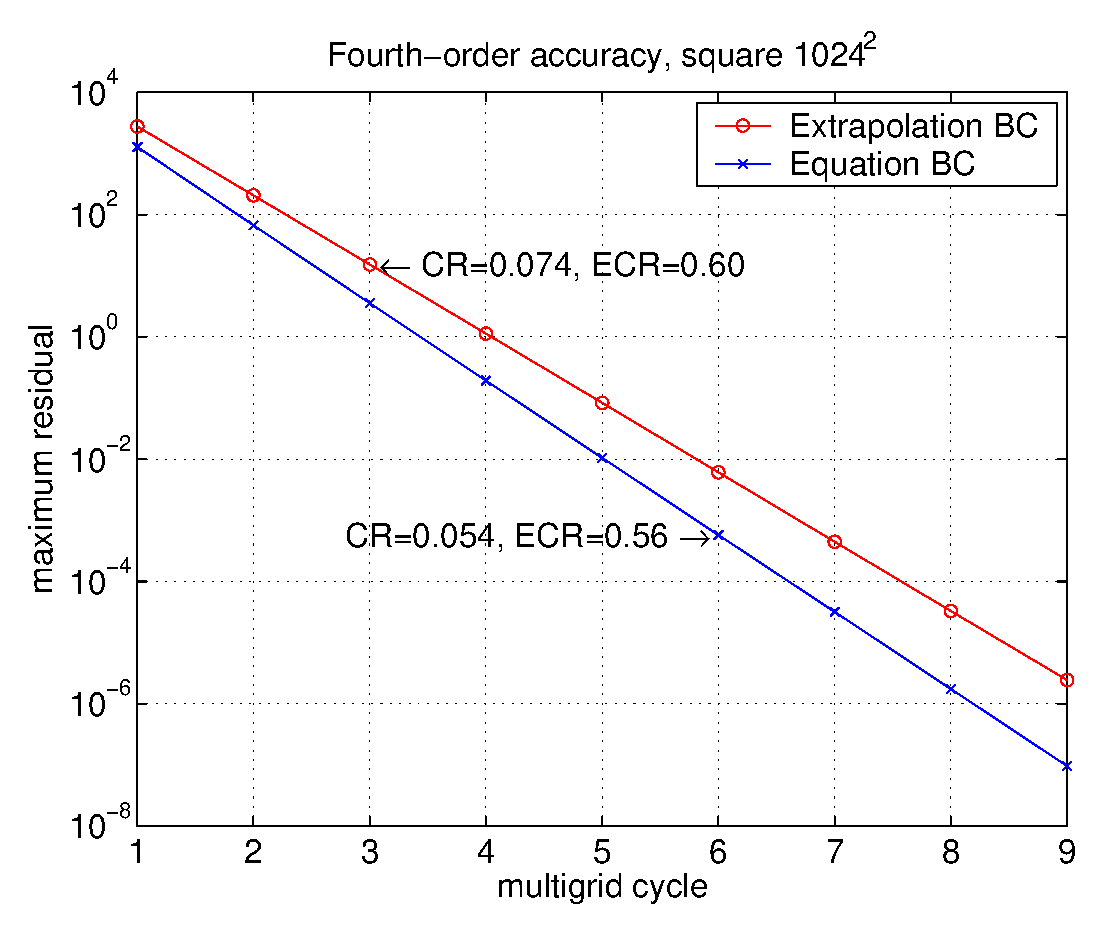
\epsfig{file=\ogmgDir/fourthOrderBC.square1024.eps,width=\figWidth}
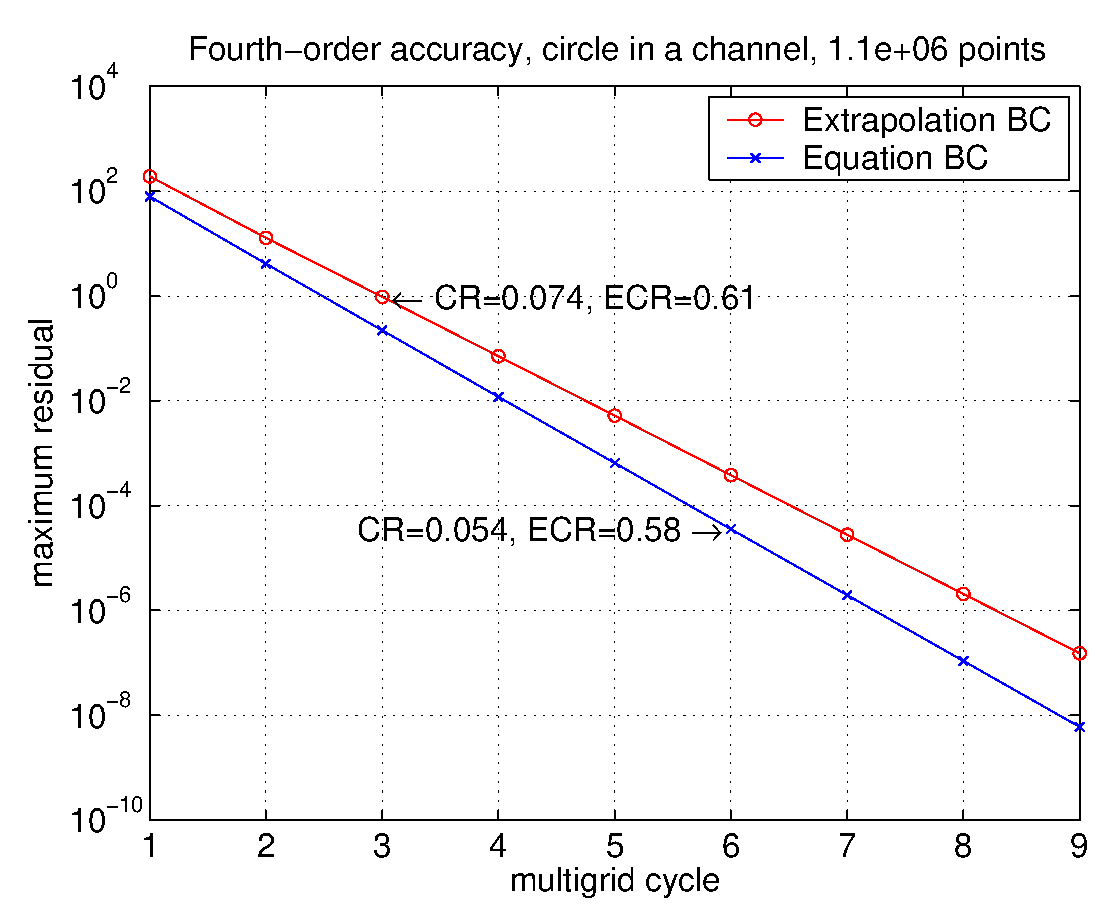
\epsfig{file=\ogmgDir/fourthOrderBC.cic6.eps,width=\figWidth}
\end{center}
\caption{A comparison of boundary conditions for the fourth-order accurate discretization.
Results are shown for a V[2,1] cycle with $\omega=1$.}
\label{fig:fourthOrderBC}
\end{figure}


\begin{table}[hbt]
\begin{center}
\begin{tabular}{|c|c|c|c|c|} \hline 
 \multicolumn{5}{|c|}{Equation BC}\\   \hline 
 $i$   & res      & rate    &  WU    & ECR  \\   \hline 
 $ 1$  & $ 3.0e+02$ & $0.048$ & $ 5.1$ & $0.55$ \\ 
 $ 2$  & $ 1.4e+01$ & $0.046$ & $ 5.1$ & $0.54$ \\ 
 $ 3$  & $ 7.0e-01$ & $0.051$ & $ 5.1$ & $0.55$ \\ 
 $ 4$  & $ 3.6e-02$ & $0.051$ & $ 5.1$ & $0.56$ \\ 
 $ 5$  & $ 1.9e-03$ & $0.052$ & $ 5.1$ & $0.56$ \\ 
 $ 6$  & $ 9.7e-05$ & $0.052$ & $ 5.1$ & $0.56$ \\ 
 $ 7$  & $ 5.1e-06$ & $0.053$ & $ 5.1$ & $0.56$ \\ 
\hline 
\end{tabular} \qquad
\begin{tabular}{|c|c|c|c|c|} \hline 
 \multicolumn{5}{|c|}{Extrapolation BC}\\   \hline 
 $i$   & res      & rate    &  WU    & ECR  \\   \hline 
 $ 1$  & $ 1.1e+03$ & $0.104$ & $ 5.1$ & $0.64$ \\ 
 $ 2$  & $ 7.3e+01$ & $0.069$ & $ 5.1$ & $0.59$ \\ 
 $ 3$  & $ 5.4e+00$ & $0.074$ & $ 5.1$ & $0.60$ \\ 
 $ 4$  & $ 3.9e-01$ & $0.073$ & $ 5.1$ & $0.60$ \\ 
 $ 5$  & $ 2.9e-02$ & $0.074$ & $ 5.1$ & $0.60$ \\ 
 $ 6$  & $ 2.1e-03$ & $0.074$ & $ 5.1$ & $0.60$ \\ 
 $ 7$  & $ 1.6e-04$ & $0.074$ & $ 5.1$ & $0.60$ \\ 
\hline 
\end{tabular}\\
\end{center}
\caption{Fourth-order accuracy with dirichlet boundary conditions. Left: Using the equation BC. Right: using extrapolation. Multigrid convergence rates, 5 levels, smoother rb[2,1]. Grid square256.order4, trigonometric solution.}
\label{tab:boundaryConditions4} 
\end{table}

% results from cic.results and newTables.tex
% run: ob/conv/cr cic.results
\begin{table}[hbt]
\begin{center}
\begin{tabular}{|c|c|c|c|} \hline 
 \multicolumn{4}{|c|}{Fourth-Order Convergence Results}\\   \hline 
 grid         &   $h/h_0$  & error (eq)  & error (extrap)   \\   \hline 
 cic.order4   &   1/1      & 1.58e-06  & 1.03e-05       \\ 
 cic2.order4  &   1/2      & 1.03e-07  & 7.02e-07       \\ 
 cic3.order4  &   1/4      & 6.51e-09  & 4.51e-08       \\ 
 cic4.order4  &   1/8      & 4.09e-10  & 2.84e-09       \\ \hline 
  rate        &              &  3.97     & 3.94  \\ \hline   
\end{tabular} \qquad
\end{center}
\caption{Maximum errors and convergence rate in the computed solution for a sequence of circle-in-a-channel grids.
   Poisson's equation is solved with the fourth-order accurate discretization and the ``equation'' or
``extrapolation'' numerical 
boundary condition. Both boundary conditions are fourth-order accurate but the ``equation'' boundary condition
gives more accurate results and converges faster.}
\label{tab:fourthOrderAccuracy} 
\end{table}



% ==========================================================
\clearpage
\subsection{Fourth-order Neumann boundary conditions}


For a Neumann boundary condition we proceed in a similar way as for the dirichlet case. For Poisson's
equation on a rectangular grid,
\begin{align*}
   u_{xx} + u_{yy} &= f \\
   u_x(0,y) & = g(y) \qquad \mbox{at $x=0$}
\end{align*}
we apply the boundary operator to the interior equation on the boundary giving
\[
   u_{xxx}(0,y) = - g_{yy}(0,y) + f_x(0,y)\qquad \mbox{at $x=0$}
\]
This equation can be discretized to second-order accuracy to give a numerical boundary condition.
In addition we apply the Neumann boundary condition to fourth-order on the boundary and
the interior equation to fourth-order on the boundary. 

In particular, on a rectangular grid we use the approximations
 \begin{align}
  D_{0x}( I - {h_x^2\over6} D_{+x}D_{-x}) U_\iv &= g(y) \\
  D_{0x} D_{+x}D_{-x} U_\iv &= - g_{yy}(0,y) + f_x(0,y) \quad := F(y)
\end{align}
and thus 
\[
   D_{0x}U = g(y) + {h_x^2\over6}F(y) 
\]
This gives
\begin{align}
    U_{-1} &= U_{+1} - 2 h_x g(y) - {h_x^3\over3} F  \\
    U_{-2} &= U_{+2} - 4 h_x g(y) - {8\over3}h_x^3 F  
\end{align}
   
\newcommand\norm[1]{\vert\vert#1\vert\vert}

On a general curvilinear grid, the mixed boundary condition is 
\[
  \alpha_0 u + \alpha_1 u_n = g
\]
or with $\nv=(n_1,n_2)$,
\[
  \alpha_0 u +\alpha_1 \Big( n_1( r_x u_r + s_x u_s ) + n_2 ( r_y u_r + s_y u_s ) \Big) = g
\]
On the boundary $r=0$ or $r=1$ the outward 
normal is $\nv = \sigma \grad_\xv r / \norm{\grad_\xv r} $ where $\sigma=\pm 1$
while at $s=0$ or $s=1$ the normal is $\nv = \sigma \grad_\xv s/ \norm{\grad_\xv s} $,
and thus
\begin{align}
  \alpha_0 u +\sigma\alpha_1 \Big( (r_x^2+r_y^2) u_r + (r_x s_x+ r_y s_y) u_s \Big)/\norm{\grad_\xv r} & = g \qquad\mbox{at $r=0,1$} \\
  \alpha_0 u +\sigma\alpha_1 \Big( (r_x s_x+ r_y s_y) u_r + (s_x^2+s_y^2) u_s \Big)/\norm{\grad_\xv s} & = g \qquad\mbox{at $s=0,1$}
\end{align}



Now consider a problem on a general curvilinear grid with boundary at $r=0$, 
\begin{align}
   L u &:= c_{11} u_{rr} + c_{12} u_{rs} + c_{22} u_{ss} + c_1 u_r + c_2 u_s + c_0 u = f \label{eq:bcna}\\
   B u &:= a_1 u_r + a_2 u_s + a_0 u = g \qquad \mbox{at $r=0$} \label{eq:bcnb}
\end{align}
The numerical boundary condition can be derived from the composite operator $BL u = Bf$
or in this case more simply from $\partial_r L u = \partial_r f$,
\begin{align}
\partial_r L u &= c_{11} u_{rrr} + c_{12} u_{rrs} + c_{22} u_{rss} + c_1 u_{rr} + c_2 u_{rs} + c_0 u_r \\
               &+ \partial_r c_{11} u_{rr} + \partial_r c_{12} u_{rs} + \partial_r c_{22} u_{ss} + 
                  \partial_r c_1 u_r + \partial_r c_2 u_s + \partial_r c_0 u  = \partial_r f
\end{align}
Dividing this last expression by $c_{11}$ and rearranging gives 
\begin{align}
  u_{rrr} + c_{11}^{-1}(c_1+ \partial_r c_{11}) u_{rr}
                & = - c_{11}^{-1}\Big[ c_{12} u_{rrs} + c_{22} u_{rss}  + c_2 u_{rs} + c_0 u_r 
                              + \partial_r c_{12} u_{rs}\\
          &\qquad  + \partial_r c_{22} u_{ss} + \partial_r c_1 u_r + \partial_r c_2 u_s + \partial_r c_0 u\Big]
                      +c_{11}^{-1}\partial_r f  \label{eq:nbc}
\end{align}
From this last equation we use the PDE (\ref{eq:bcna}) and boundary condition (\ref{eq:bcnb})
to derive an expression of the form
\begin{align}
 u_{rrr} + b_{11} u_{rr} &= b_0 u + b_1 u_s + b_3 u_{sss} + b_f \label{eq:numBC}
\end{align}
We will discretize (\ref{eq:numBC}) to second-order and use it as the numerical boundary condition.
I guess that $b_1$ and $b_3$ are zero if the grid is orthogonal (check this).

We now describe how we simplify (\ref{eq:nbc}) to obtain (\ref{eq:numBC}).
From the Neumann boundary condition~(\ref{eq:bcnb}) we know $u_r$ on the boundary,
\begin{align}
    u_r(0,s) & := G(s) \\
             & =   a_1^{-1} ( g - a_2 u_s - a_0 u ),  \qquad \mbox{at $r=0$} \\
\end{align}


Better? Differentiating the expression for $u_r$ with respect to the tangential variable $s$
gives 
\begin{align}
   u_{rs}(0,s) & := G_s(s) \\
               & = a_1^{-1} \Big( g_s - a_2 u_{ss} - a_0 u_s - (\partial_s a_2) u_s - (\partial_s a_0) u \\
               &\qquad      -(\partial_s a_1) a_1^{-1} ( g - a_2 u_s - a_0 u ) \Big),  \qquad \mbox{at $r=0$} \\
   u_{rss}(0,s) & := G_{ss}(s)
\end{align}

This last expression can be differentiated with respect to $s$ to give
the tangential derivatives of $u_r$ on the boundary,
\begin{align}
   u_{rs}(0,s) & = G_s(s) \\
   u_{rss}(0,s) & = G_{ss}(s) \\
   G_s(s) &= a_1^{-1}\Big( g_s - [ a_2 u_{ss}+(a_0+\partial_s a_2)u_s + \partial_s a_0 u]
                               -\partial_s a_1 G(s) \Big)  \\
   G_{ss}(s) &= a_1^{-1}\Big( 
                  g_{ss} - [ a_2 u_{sss}+(a_0+2\partial_s a_2)u_{ss} 
                           +(2\partial_s a_0+\partial_s^2 a_2)u_s+ \partial_s^2 a_0 u] \\
             &~                  -\partial_s^2 a_1 G(s) - 2 \partial_s a_1 G_s(s) \Big)  
\end{align}
From the equation~(\ref{eq:bcna}) we know $u_{rr}$ on the boundary as
\begin{align}
u_{rr}(0,s) & := F(s) \\
            & = c_{11}^{-1} \Big[ f - (c_{12} u_{rs} + c_{22} u_{ss} + c_1 u_r + c_2 u_s + c_0 u) \Big] \\
            & = c_{11}^{-1} \Big[ f - (c_{12} G_s(s) + c_{22} u_{ss} + c_1 G(s) + c_2 u_s + c_0 u) \Big]  
\end{align}
Thus we also know the tangential directives of $u_{rr}$,
\begin{align}
u_{rrs}(0,s) & = F_s(s) \\
  F_s(s) & = c_{11}^{-1} \Big[ f_s - \Big(c_{12} G_{ss} + (c_1+\partial_s c_{12})G_s
           + c_{22} u_{sss} + (\partial_s c_{22}+c_2)u_ss \\
         &~ +\partial_s c_1 G + 
             (\partial_s c_2 + c_0) u_s + \partial_s c_0 u\Big) -\partial_s c_{11} F \Big]
\end{align}

\newcommand{\Fs}{{\cal F}}
We can therefore write $u_{rrr}$ on the boundary from equation~(\ref{eq:nbc})
as a function of the values of u on the boundary (including
tangential derivatives of $u$),
\begin{align}
u_{rrr} & := \Fs(s) \\
        & = c_{11}^{-1}\Big[ f_r - ( c_{12} F_s(s) + c_{22} G_{ss}(s) + c_1 F(s) + c_2 G_s(s)+ c_0 G(s) \\
        & + \partial_r c_{11} F(s) + \partial_r c_{12} G_s(s) + \partial_r c_{22} u_{ss} + 
                  \partial_r c_1 G(s) + \partial_r c_2 u_s + \partial_r c_0 u \Big] 
\end{align}

Better: We can therefore write $u_{rrr}$ on the boundary from equation~(\ref{eq:nbc})
as a function of $u$ and its tangential derivatives,
\begin{align}
u_{rrr} & := \Fs(s) \\
        & =  b_0 u + b_1 u_{s} + b_2 u_{ss} + b_3 u_{sss} + f_0
\end{align}


We use the approximations
\begin{align}
  D_{0r}( I - {h_r^2\over6} D_{+r}D_{-r}) U_\iv &= G(s) \\
  D_{0r} D_{+r}D_{-r} U_\iv &= \Fs(s) 
\end{align}
and thus 
\[
   D_{0r}U = G(s) + {h_r^2\over6}\Fs
\]
This gives
\begin{align}
    U_{-1} &= U_{+1} - 2 h_r G(s) - {h_r^3\over3}\Fs \\
    U_{-2} &= U_{+2} - 4 h_r G(s) - {8\over3}h_r^3\Fs 
\end{align}
    

% ==============================================================================================

\input cornerBoundaryConditions.tex


% ==============================================================================================
\clearpage

\subsection{Boundary conditions and eigenfunctions}


In order to understand how to choose numerical boundary conditions,
it is instructive to consider the eigenvalue problem
corresponding to the elliptic boundary value problem.
Consider the eigenvalue problem for Laplace's equation on a square with Dirichlet
boundary conditions.
\begin{align*}
   - \Delta u & = \lambda u \qquad \xv\in\Omega := [0,1]^d \\
    u&=0  \qquad  \xv\in\partial\Omega   
\end{align*}
At the boundary $x=0$ we know that $u(0,y)=0$. From the PDE we also
know that 
\begin{align*}
  u_{xx}(0,y) &= - u_{yy}(0,y) + \lambda u(0,y) \\
              & = 0
\end{align*}
By differentiating the PDE an even number of times with respect to $x$ we see that all
\begin{align*}
  \partial_x^{2p} u(0,y) &= 0 \qquad p=1,2,\ldots \qquad\mbox{(Dirichlet boundary)}
\end{align*}
and thus the eigenfunction $u$ is an odd function of $x$ about $x=0$. 
Indeed $u$ is an odd function about each of the boundaries. 
This leads us to reason that the discrete boundary conditions we choose for the
a Dirichlet boundary should be chosen to preserve this odd symmetry so that the discrete
eigenfunctions will also have this symmetry. 

In the case of Neumann boundary conditions it is easy to see that all odd derivatives will
be zero at the boundary
\begin{align*}
  \partial_x^{2p-1} u(0,y) &= 0 \qquad p=1,2,\ldots\qquad\mbox{(Neumann boundary)}
\end{align*}
and thus the eigenfunction $u$ is an even function of $x$ about the boundary $x=0$.
The discrete boundary for a Neumann boundary condition should preserve this symmetry.
In the simple case of a rectangular grid on a square, the discrete eigenfunctions
are basically the same as the continuous ones provided the Neumann boundary condition
is discretized appropriately. In then follows that local Fourier analysis is actually
valid for the problem with boundaries. As a result, the smoothing rates and
convergence factors for Neumann boundary conditions should be basically the same as those
for Dirichlet boundary conditions.

\subsubsection{Discrete eigenfunctions in one-dimension}

Consider the one-dimensional eigenvalue problem
\begin{align}
   - u_{xx} & = \lambda u \qquad x\in (0,1)\\
      u(0)&=u(1)=0
\end{align}
The eigenvalues $\lambda^{(e)}_m$ and eigenvectors $u^{(e)}_m$ are
\begin{align}
     \lambda^{(e)}_m &= (m \pi)^2 \qquad m=1,2,\ldots \\
      v^{(e)}_m &= \sin( \pi m x ) \label{eq:ctseiv}
\end{align}
We discretize this problem using fourth-order accurate difference approximations,
method:
\begin{align}
   -  D_+ D_-( 1 - {h^2\over 12} D_+ D_- ) U_i & = \lambda U_i \qquad i=1,2,3,\ldots,N-1 \label{eq:pde4}\\
      U_0 &=0    \\ 
      U_N &= 0   
\end{align}
on the grid $x_i = i h$, $h=1/N$.
Later in this section we show that good numerical bounday conditions are given by
the equations discretized to second-order on the boundary:
\begin{align}
    D_+ D_- U_0 &= 0     \label{eq:eqBC}\\
    D_+ D_- U_N &= 0 ~.
\end{align}
With these boundary conditions we can solve the eigenvalue problem explicitly giving
eigenvalues $\lambda_m$ and eigenfunctions $U_i^{(m)}$,
\begin{align}
  \lambda_m &= {4\over h^2} \Big[ \sin^2(\xi_m)+ {1\over 3} \sin^4(\xi_m) \Big] \qquad m=1,2,\ldots,N-1\\
    \xi_m &= \pi m h/2 \\
  U_i^{(m)} &= \sin( \pi m x_i )   \label{eq:eiv}
\end{align}
For $ m h \ll 1 $ we see that the eigenvalues are fourth order accurate,
\begin{align*}
  \lambda_m &= {4\over h^2} \Big[ (\xi_m - {1\over6}\xi_m^3)^2 + {1\over 3}\xi_m^4 \Big] +O(h^{-2} \xi_m^6) \\
            &= {4\over h^2} \xi_m^2  + O(h^{-2}\xi_m^6) \\
            &= (m \pi)^2  + O(m^6 h^4) \\
\end{align*}            
Note that the discrete eigenvectors (\ref{eq:eiv}) are exactly the same as the
continuous eigenvectors.

Now consider using extrapolation boundary conditions in place of (\ref{eq:eqBC}),
\begin{align}
    D_+^p U_0 &= 0     \label{eq:extrapBC}\\
    D_-^p U_N &= 0 ~.
\end{align}
We can choose $p=4$ to obtain fourth-order accuracy.
The solution to the eigenvalue/eigenfunction problem is more complicated in this case.
Making the anstaz
\[
    U_i = \kappa^i
\]
and substituting into \ref{eq:pde4} gives
\[
    (\kappa-2+\kappa^{-1})(1 - {1\over12}(\kappa-2+\kappa^{-1}) ) = -\lambda h^2
\]
Letting $z=-(\kappa-2+\kappa^{-1})$ we see that $z$ satifies the quadratic equation
\[
      z^2 + 12 z - 12 \lambda h^2 = 0
\]
with roots
\begin{align*}
      z_\pm &= -6 \pm \sqrt{ 6^2 + 12 \lambda h^2 } \\
            &= 6\Big( -1 \pm \sqrt{ 1 + {1\over3} \lambda h^2 } ~\Big)
\end{align*} 
where 
\begin{align*}
    z_1 &=6\Big( -1 + \sqrt{ 1 + {1\over3} \lambda h^2 } ~\Big) \\
        &=  \lambda h^2 + O( \lambda^2 h^4) \\
    z_2 &= 6\Big( -1 - \sqrt{ 1 + {1\over3} \lambda h^2 } ~\Big) \\
        & = -12 - \lambda h^2 + O( \lambda^2 h^4)
\end{align*}
Note that for $\lambda\in\Real$ and $\lambda>0$ we have $|z_2|>12$. For $\lambda\in{\Bbb C}$,
$|z_2|\ge 6$.

Given $z$ we solve for $\kappa$ from $\kappa^2-2(1-z/2)\kappa+1=0$,
\[
    \kappa = 1-{1\over2}z \pm \sqrt{ (1-{1\over2}z)^2 -1 }
\]
with
\begin{align*}
   \kappa_1 &= 1-{1\over2}z_1 + \sqrt{ - z_1 + z_1^2/4 }    
            \quad = 1 + \sqrt{-z_1} - z_1/2 +O(z_1^{3/2})  \\
            &= 1 + i\sqrt{\lambda} h - \lambda h^2 +O(z_1^{3/2})\\ 
   \kappa_2 &= 1-{1\over2}z_1 - \sqrt{ - z_1 + z_1^2/4 }    
            \quad = 1 - \sqrt{-z_1} - z_1/2 +O(z_1^{3/2})  \\
            &= 1 - i\sqrt{\lambda} h - \lambda h^2 +O(z_1^{3/2})\\ 
   \kappa_3 &= 1-{1\over2}z_2 + \sqrt{ (1-{1\over2}z_2)^2 -1 }   
            \quad = 7 + 4\sqrt{3} + O(\lambda h^2) \\
            &\approx 14   \\        
   \kappa_4 &= 1-{1\over2}z_2 - \sqrt{ (1-{1\over2}z_2)^2 -1 }    
            \quad = 7 - 4\sqrt{3} + O(\lambda h^2) \\
            &\approx {1\over 14} 
\end{align*}
where $\kappa_1\kappa_2=1$, $\kappa_3\kappa_4=1$.

The roots $\kappa_1$ and $\kappa_2$ correspond to the physical solutions,
\begin{align*}
   \kappa_1^i =& e^{ i \lambda x_i} + O()\\
   \kappa_2^i =& e^{-i \lambda x_i} + O()\\
\end{align*}
while the roots $\kappa_3$ and $\kappa_4$ are spurious.

There are four roots, $\kappa_m$, $m=1,2,3,4$ to this equation
and the general solution will be of the form
\[
   U_i = \sum_{m=1}^4 \alpha_m \kappa_m^i
\]

Applying the boundary conditions,
\begin{align}
     \alpha_1 + \alpha_2 + \alpha_3 + \alpha_4 &= 0 \label{eq:eiv1}\\
     \alpha_1\kappa_1^N + \alpha_2\kappa_2^N + \alpha_3\kappa_3^N + \alpha_4\kappa_4^N &= 0\label{eq:eiv2} \\
\end{align}
With the $D_+D_-U_0=0$ BC's we also have
\begin{align}
  \alpha_1 z_1 + \alpha_2 z_1 + \alpha_3 z_2 + \alpha_4 z_2 &= 0  \label{eq:eiv3}\\
  \alpha_1 z_1\kappa_1^N + z_1\alpha_2\kappa_2^N + \alpha_3 z_2\kappa_3^N + \alpha_4 z_2\kappa_4^N &= 0 \label{eq:eiv4}
\end{align}
Taking $z_2$ times (eq:eiv1) minus (eq:eiv3)  and ... gives
\begin{align}
  \alpha_1 + \alpha_2 &= 0 \\
  \alpha_1 \kappa_1^N + \alpha_2\kappa_2^N &=0 
\end{align}
There is a non-trivial solution to this problem, $A\alpha=0$, provided the determinant of $A$ is
zero.
The determinant is 
\[
  |A| =  - (z_2-z_1)^2 (\kappa_1^N - \kappa_1^{-N})(\kappa_3^N - \kappa_3^{-N})
\]
There is a non-trivial solution to this problem provided
\begin{align}
  \kappa_1^{2N} &=1 
\end{align}
NOTE: also the possibility that $\kappa_3^{2N}=1$ but this is not possible since $|\kappa_{3}|>1$. 
We are thus led to $\alpha_1=-\alpha_2$, $\alpha_{3,4}=0$,
and therefore
\[
   U_i = \alpha_1 (\kappa_1^i - \kappa_1^{-i} )
\]


Now consider the extrapolation BC's $D_+^4 U_0=0$. Using $D_+^4\kappa_m^i = D_+D_-\kappa_m^{i+2}$ gives
\begin{align}
  \alpha_1 z_1 \kappa_1^2 + \alpha_2 z_1 \kappa_2^2
                    + \alpha_3 z_2\kappa_3^{2} + \alpha_4 z_2\kappa_4^{2} &= 0  \label{eq:eiv3}\\
  \alpha_1 z_1\kappa_1^{N-2} + z_1\alpha_2\kappa_2^{N-2} 
                    + \alpha_3 z_2\kappa_3^{N-2} + \alpha_4 z_2\kappa_4^{N-2} &= 0 \label{eq:eiv4}
\end{align}
or
\begin{align}
  \alpha_1  + \alpha_2 \kappa_2^4 + \alpha_3 z_2\kappa_3^{2}z_1^{-1}\kappa_1^{-2}
                 + \alpha_4 z_2\kappa_4^{2}z_1^{-1}\kappa_1^{-2} &= 0  \label{eq:eiv3}\\
  \alpha_1  + \alpha_2 z_1\kappa_2^{2N-4} 
                 + \alpha_3 z_2\kappa_3^{N-2}z_1^{-1}\kappa_1^{N-2} 
                 + \alpha_4 z_2\kappa_4^{N-2}z_1^{-1}\kappa_1^{N-2}  &= 0 \label{eq:eiv4}
\end{align}

In this case the eigenfunction is not independent of the spurious modes. Figure~(\ref{fig:fourthOrderExtrapBC}) shows 
the errors in the first 10 eigenfunctions for $N=80$ and $N=160$. The low frequency eigenfunctions have a
sharp boundary layer. 
Notice that the extrapolation condition $D_+^4 U_{-1} =0$ implies the condition $(D_+D_-)^2 U_1=0$. 


% , implies from (\ref{eq:pde4})
% that $D_+D_-U_{1} = \lambda U(1) = O(\lambda h)$. Thus extrapolation is approximately equivalent
% to imposing $u_{xx}(h)=0$ (instead of the correct condition $u_{xx}(0)=0$). 
% The eigenfunctions show this behaviour.
 It is now apparent why standard usual multigrid  smoothers
have difficulty with the extrapolation boundary condition. Suppose we expand the error in terms of the eigenfunctions,
\[
      e_i = \sum_m \beta_m U^{(m)}_i 
\]
The standard multigrid smoothers will not damp eigen-components
of the solution corresponding to low frequency eigenvalues. For example, the Jacobi smoother has operator
\[
       S_J =  I - D^{-1} L_h
\]
and therefore when applied to an eigenfunction, the amplification factor will be
\[
       \mu_J =  1 - {12\over30} h^2 \lambda^{(m)}
\]
and thus eigenfunctions with small values of $\lambda^{(m)}$ will not be changed very much.
Thus, after smoothing, the error will still have
a sharp boundary layer which will not be well represented on the coarser grids.
% since the application of the smoother and boundary conditions will generate high frequency
% components near the boundary.


\renewcommand{\figWidth}{.495\linewidth}
\begin{figure}
\begin{center}
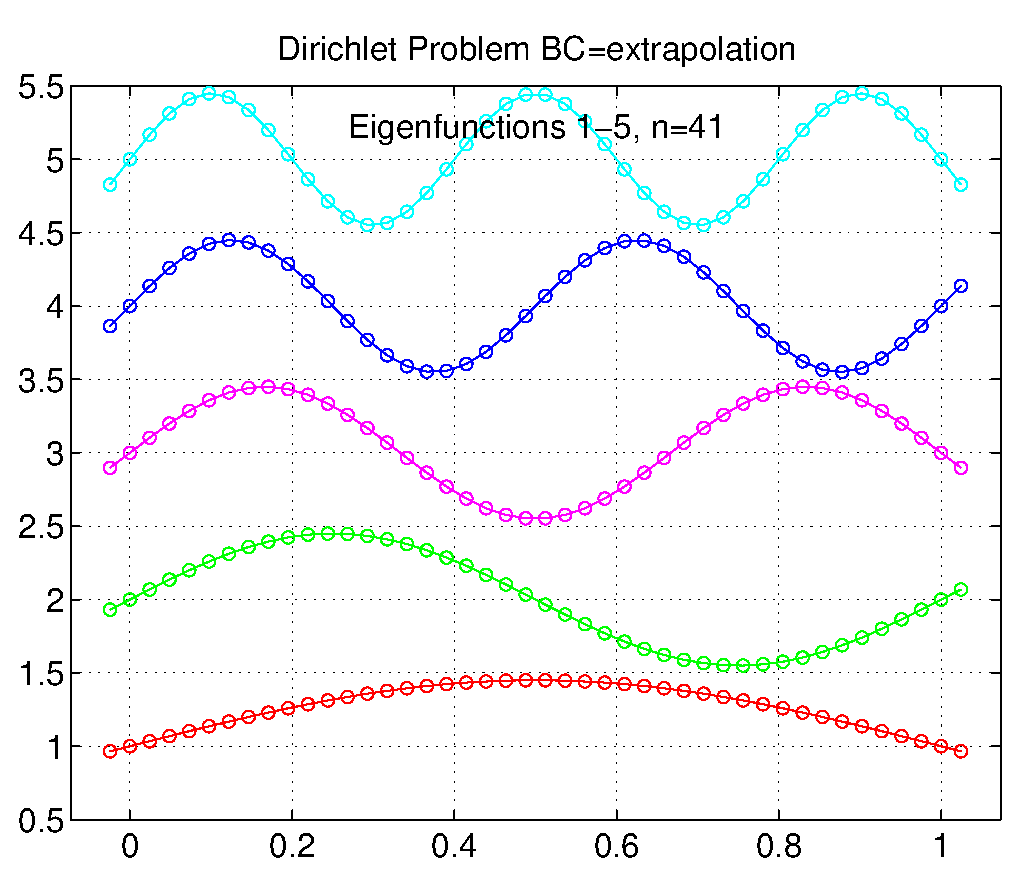
\epsfig{file=\ogmgDir/bceig-41-extrap-1.eps,width=\figWidth}
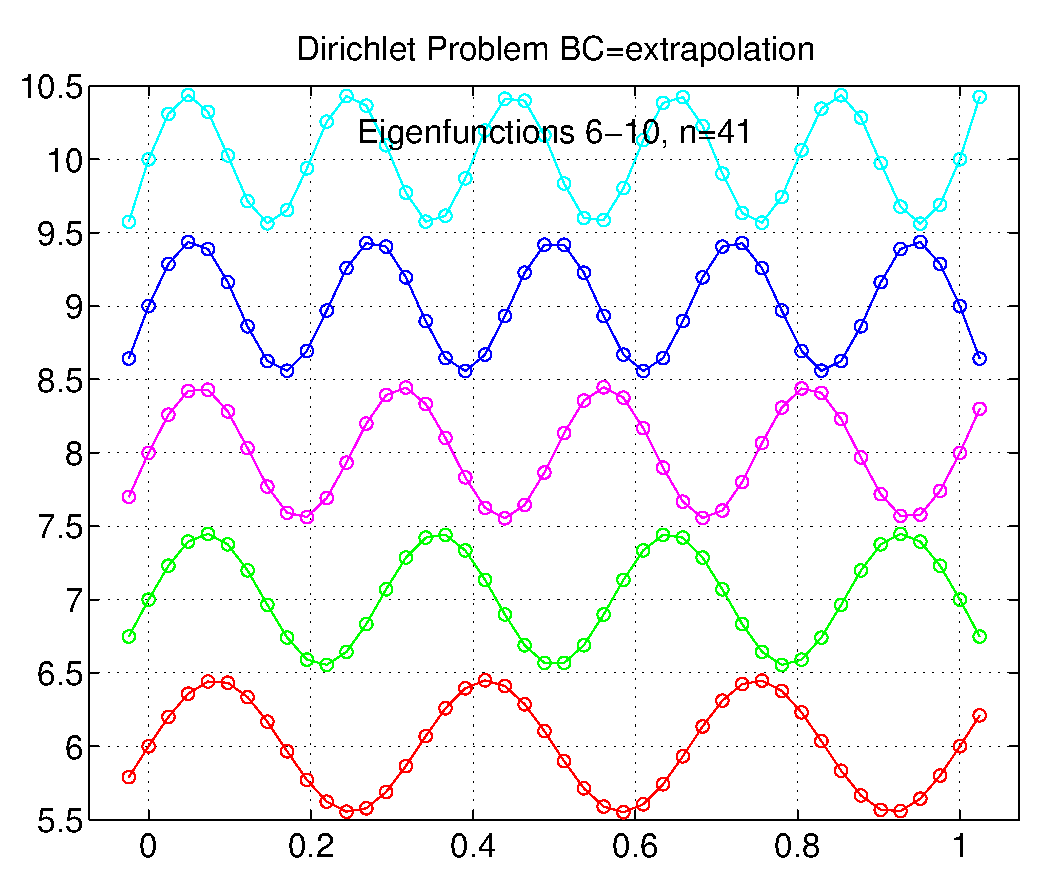
\epsfig{file=\ogmgDir/bceig-41-extrap-2.eps,width=\figWidth}
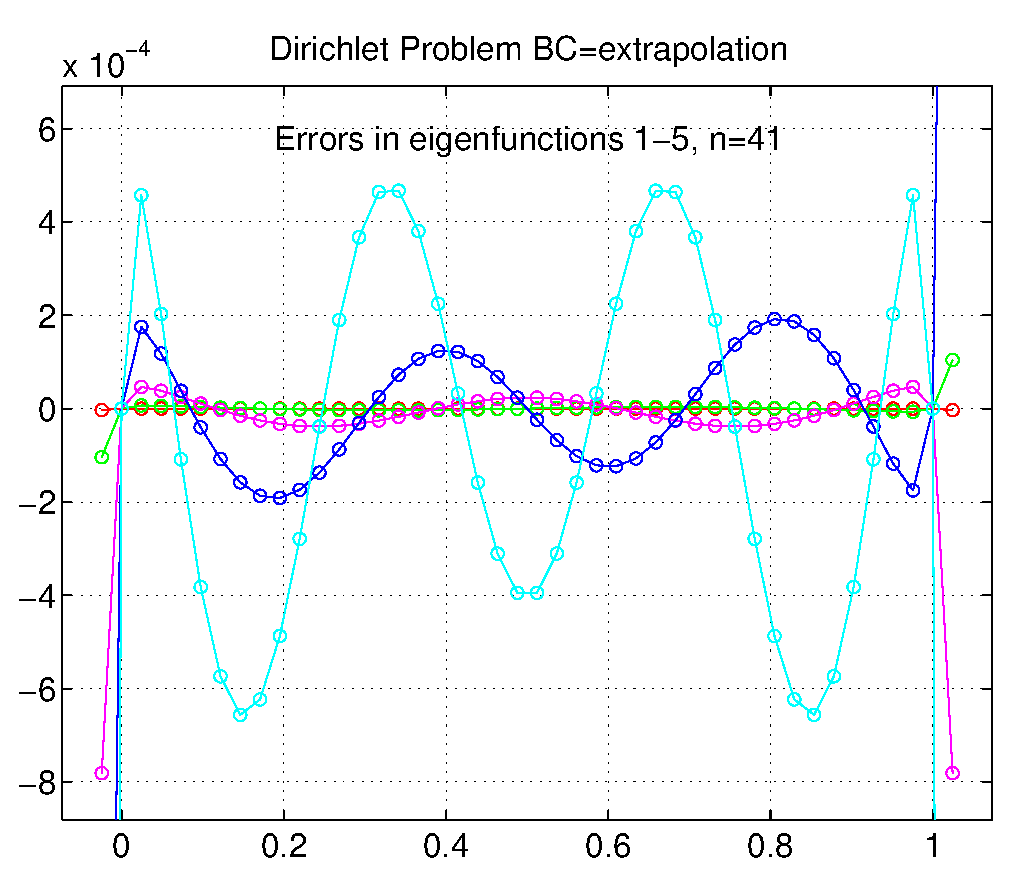
\epsfig{file=\ogmgDir/bceig-err-41-extrap-1.eps,width=\figWidth}
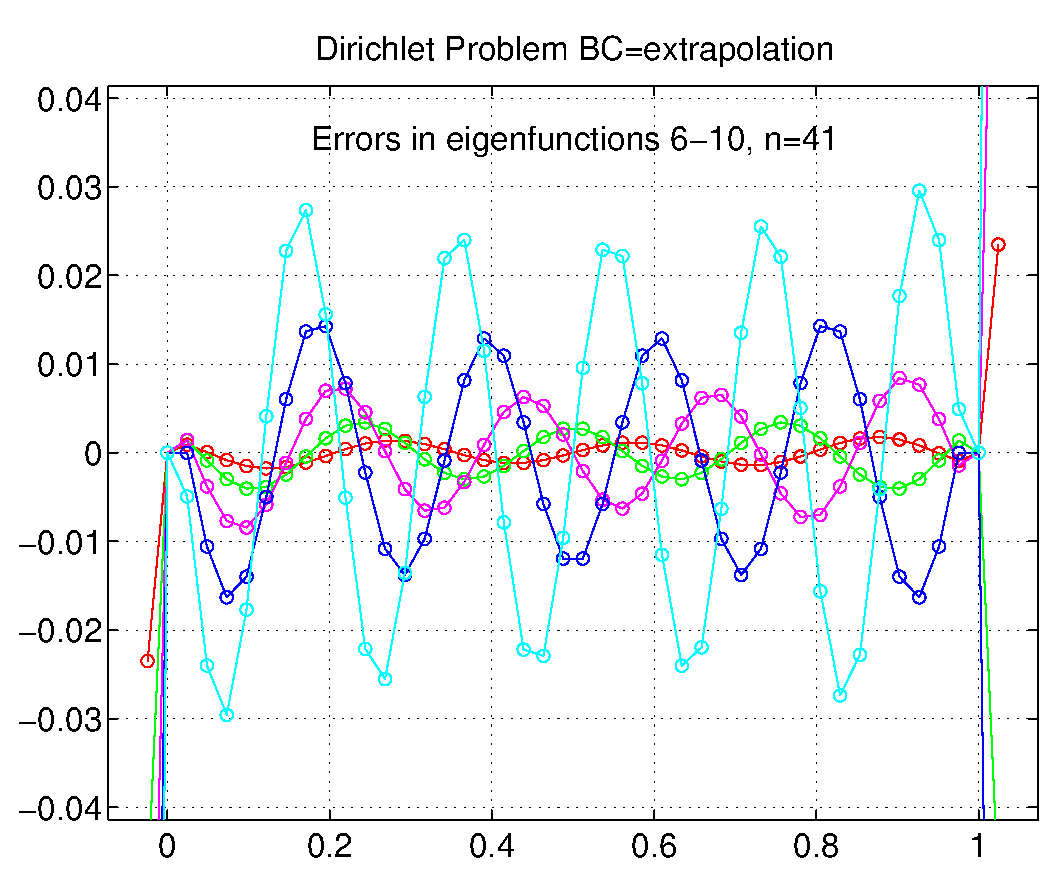
\epsfig{file=\ogmgDir/bceig-err-41-extrap-2.eps,width=\figWidth}
\end{center}
\caption{Eigenfunctions and errors in the eigenfunctions for the fourth-order accurate discretization of the Dirichlet problem
 with the $D_+^4U =0$ extrapolation BC. The solution is shown including ghost points.
 The errors are largest in a boundary layer.The value on the first ghost line may
be outside the scale shown. }
\label{fig:fourthOrderExtrapBC}
\end{figure}


\renewcommand{\figWidth}{.495\linewidth}
\begin{figure}
\begin{center}
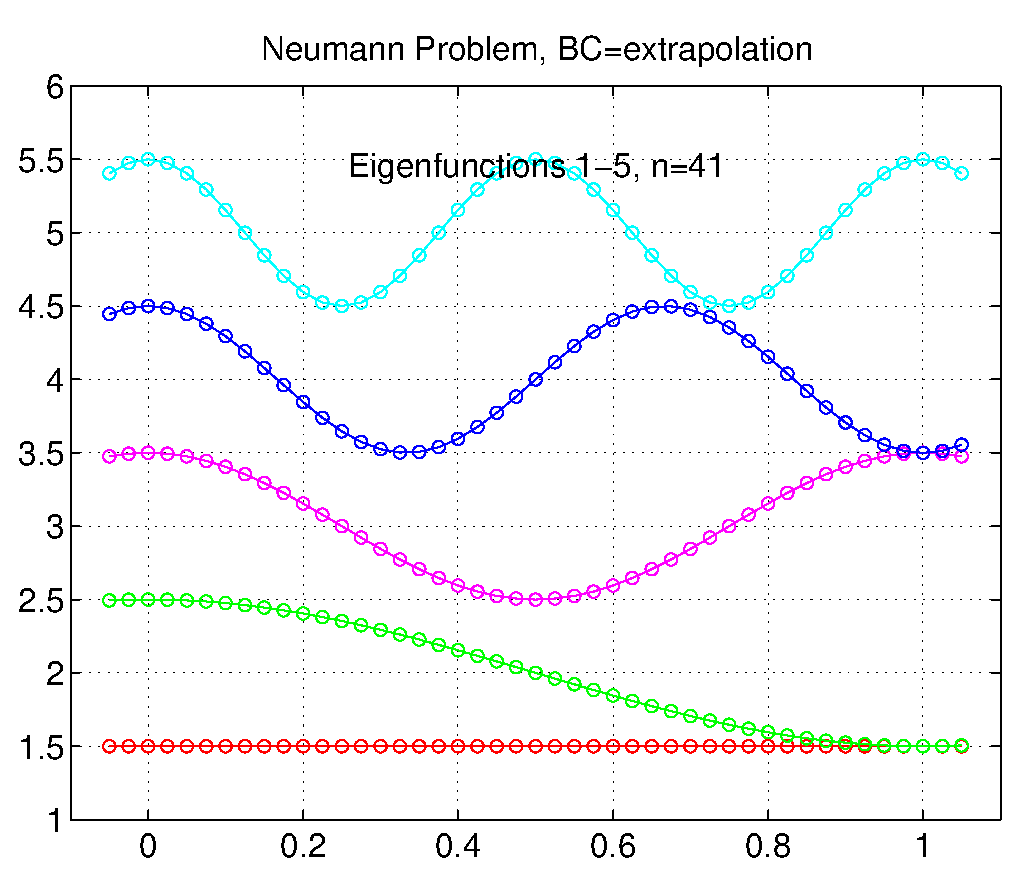
\epsfig{file=\ogmgDir/bceign-41-extrap-1.eps,width=\figWidth}
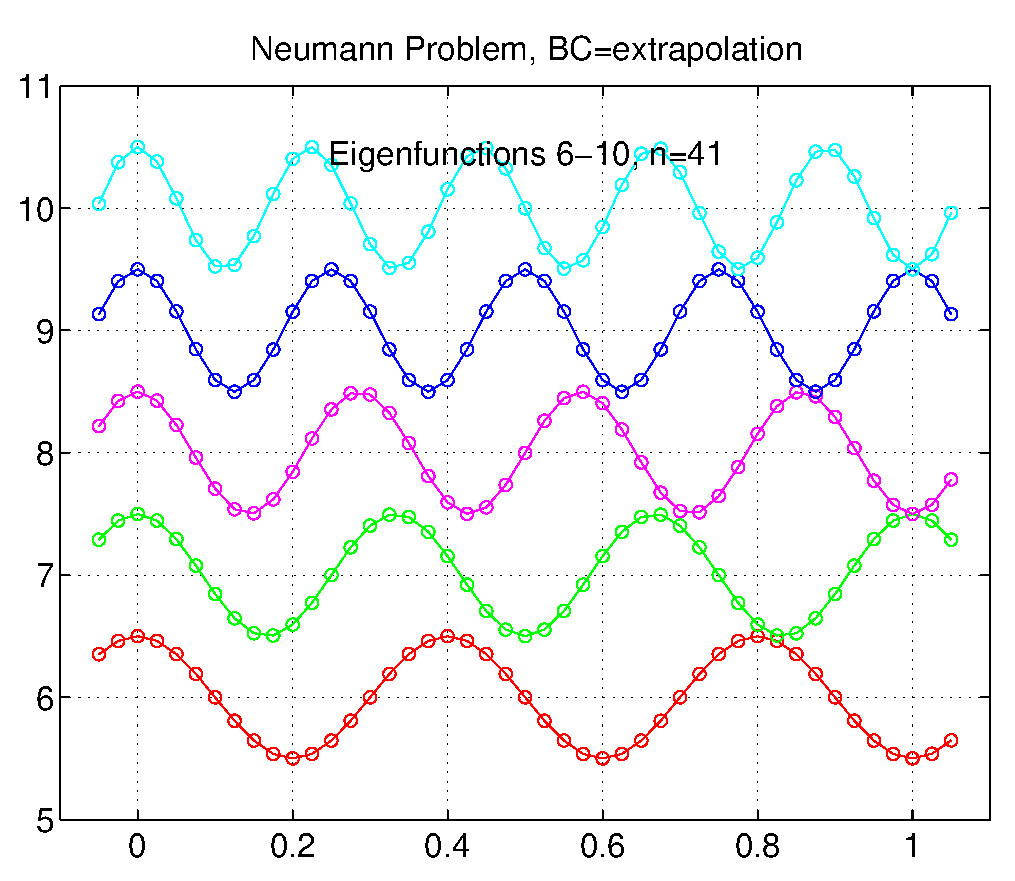
\epsfig{file=\ogmgDir/bceign-41-extrap-2.eps,width=\figWidth}
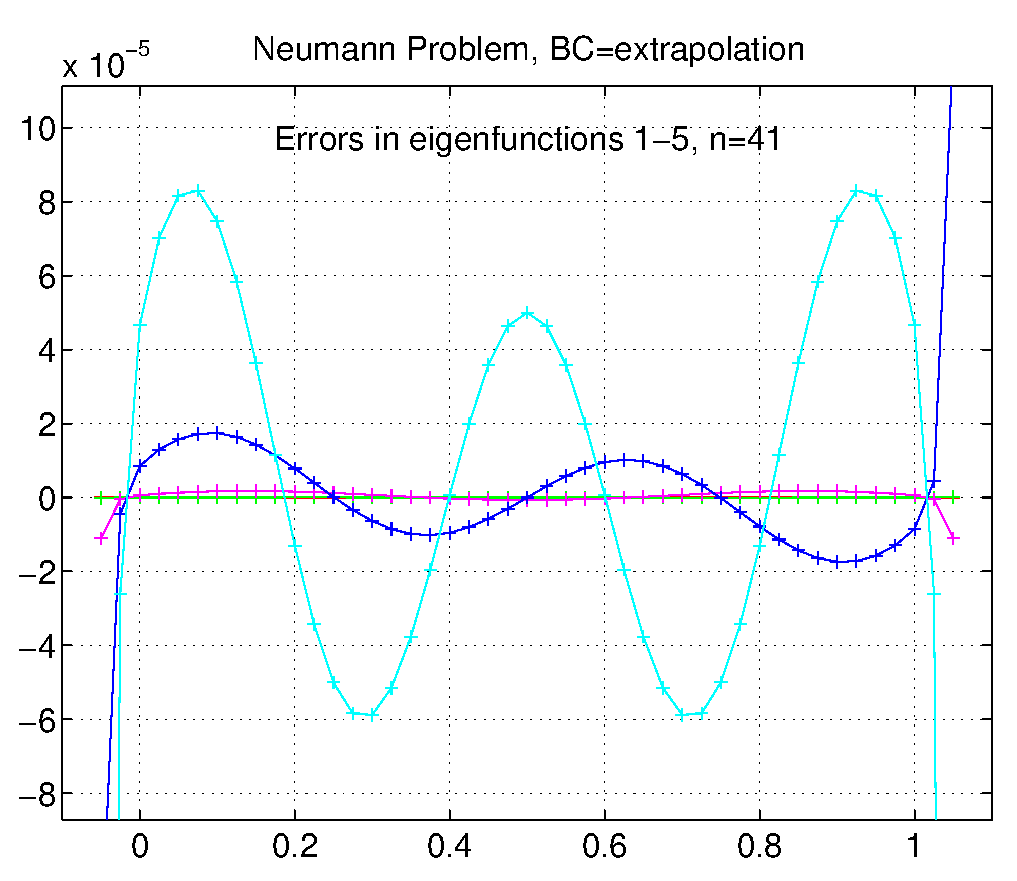
\epsfig{file=\ogmgDir/bceign-err-41-extrap-1.eps,width=\figWidth}
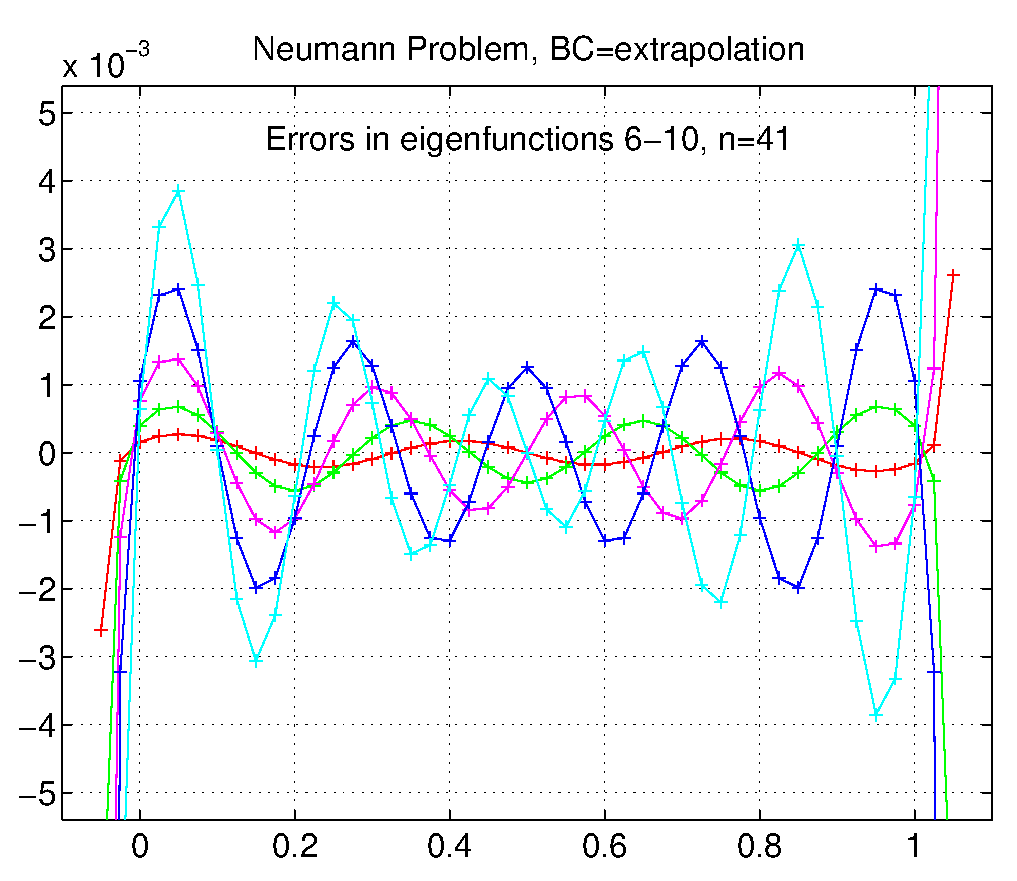
\epsfig{file=\ogmgDir/bceign-err-41-extrap-2.eps,width=\figWidth}
% 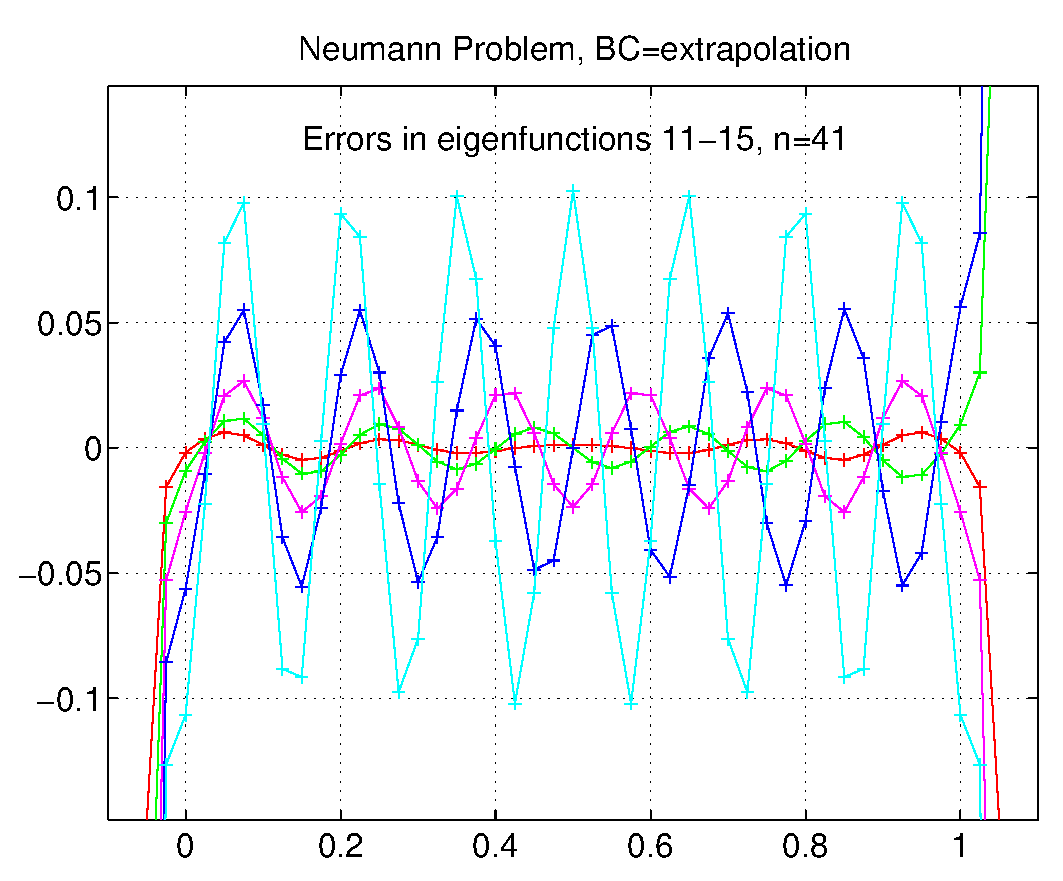
\epsfig{file=\ogmgDir/bceign-err-41-extrap-3.eps,width=\figWidth}
% 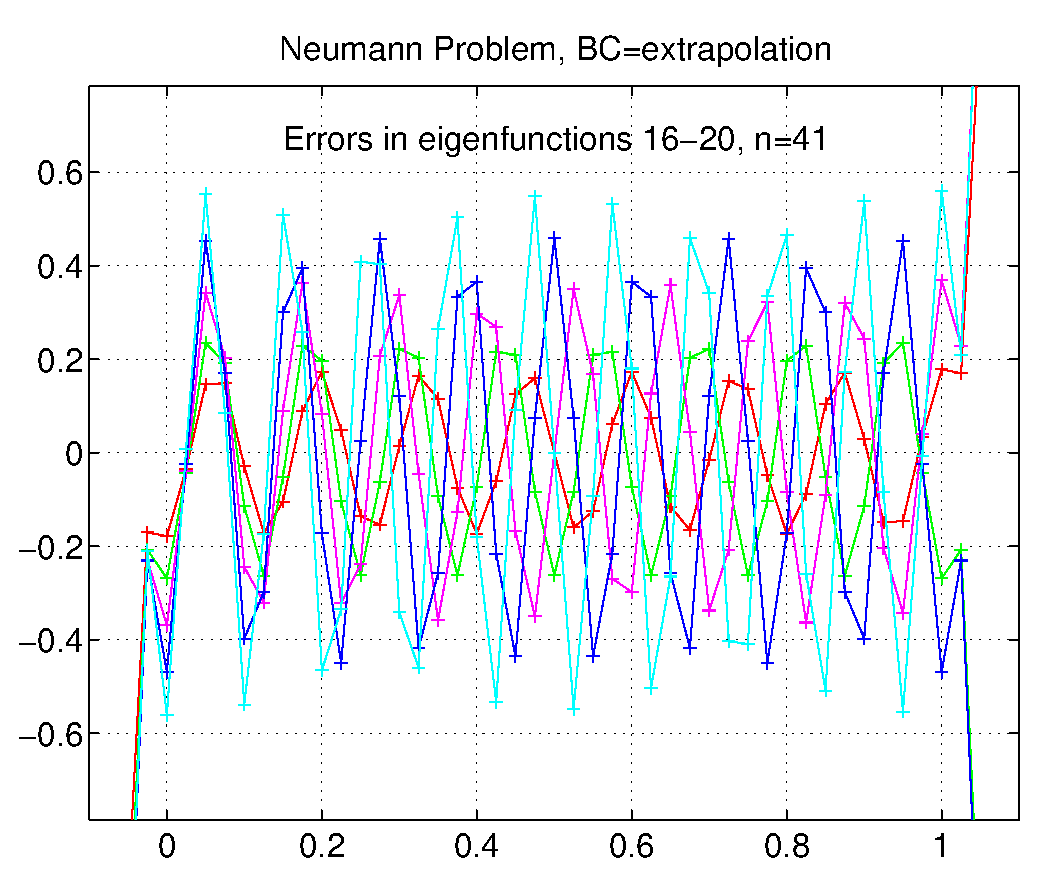
\epsfig{file=\ogmgDir/bceign-err-41-extrap-4.eps,width=\figWidth}
\end{center}
\caption{Eigenfunctions and errors in the eigenfunctions for fourth-order discretization of the Neumann problem
 with the $D_+^5U_{-2} =0$ extrapolation BC. The solution is shown including ghost points.
 The errors are largest in a boundary layer on each end. The value on the second ghost line may
be outside the scale shown.}
\label{fig:fourthOrderNeumannExtrapBC}
\end{figure}
